\documentclass[class=book, crop=false, oneside, 12pt]{standalone}
\usepackage{standalone}
\usepackage{../../style}
\usepackage{../../style_automata}
\graphicspath{{./assets/images/}}

\begin{document}

\chapter{Automi a stati finiti: teoria, algoritmi e simili amenità}

\section{Traduzione da NFA a DFA}
Abbiamo già discusso in passato di come la simulazione su DFA sia più efficiente che su NFA, quindi ora siamo interessati a risolvere questo problema: dato un qualunque NFA some si può ricavare un DFA che riconosca lo stesso linguaggio?

Un mezzo per raggiungere questo scopo è l’utilizzo di una sorta di meccanismo di \(\varepsilon\)-chiusura permanente (che elimini in modo permanente le \(\varepsilon\)-transizioni), questo meccanismo si chiama Subset Construction.


\subsection{Algoritmo di Subset Costruction}
L’algoritmo di Subset Construction serve per ricavare un DFA dato un certo NFA.

L'idea di base è quella di utilizzare la \(\varepsilon\)-chiusura per mappare sottoinsiemi degli stati del dato NFA (che in seguito chiameremo rozzamente \emph{stati non deterministici}, o \emph{snd}) in stati per il nuovo DFA (che in seguito chiameremo ancor più rozzamente \emph{stati deterministici} o \emph{sd}).

Per dare un'idea di come lavora questo algoritmo descriviamone i primi passi.\\
Si individua qual è lo stato iniziale dell'NFA, diciamo \(S_0\), lo si prende come punto di partenza e se ne calcola la \(\varepsilon\)-chiusura \(T\); sarà proprio \(T\) ad essere lo stato iniziale del DFA. Ora dovrebbe essere più chiaro quello che si fa in questo algoritmo: si eliminano tutte le \(\varepsilon\)-transizioni per ottenere un set di transizioni \(\textrm{move}_d\) che contiene solo transizioni "deterministiche".

Un fatto da tenere sempre ben presente è che gli stati del DFA che otteniamo in questo modo sono insiemi di stati dell'NFA di partenza. Il \(T\) appena descritto è un sottoinsieme degli stati dell'NFA di partenza.

Dopo questa piccola introduzione passiamo a visualizzare subito il codice dell'algoritmo di Subset Construction.

\subimport{assets/pseudocode/}{subset-construction.tex} 
\noindent Procediamo quindi ora con una spiegazione discorsiva di questo algoritmo.
\paragraph*{Input}
L'algoritmo prende come input un NFA specificato dalla tupla \(\mathcal{N} := (S, \mathcal{A}, \textrm{move}_n, s_0, F)\)

\paragraph*{Output}
L'algoritmo ritorna come output un DFA specificato dalla tupla \(\mathcal{D} := (R, \mathcal{A}, \textrm{move}_d, s_0, E)\) tale da soddisfare la seguente condizione: \(\mathcal{L}(\mathcal{D}) = \mathcal{L}(\mathcal{N})\).

\paragraph*{Introduzione}
Per prima cosa si calcola quello che sarà lo stato iniziale del DFA, ovvero \(T_0\); esso coinciderà, come già detto in precedenza, con la \(\varepsilon\)-chiusura dello stato iniziale dell'NFA \(S_0\). Una volta calcolato questo \(T_0\),  lo si inserisce nell'insieme \(R\) e lo si segna come \texttt{unmarked}.

\paragraph*{Ciclo while}
Qui inizia il corpo centrale dell'algoritmo: questo ciclo serve per iterare su tutti gli stati che si stanno inserendo mano a mano nell'insieme \(S\) degli stati del DFA. 

Di fatto, dentro al ciclo si scorrono tutti gli stati in \(R\) e ci si sofferma sugli stati \(T \in R\) segnati come \texttt{unmarked}. Di volta in volta, quando se ne identifica uno, lo si marca, dimodoché non venga più elaborato in seguito, quindi si procede con le successive istruzioni.

\paragraph*{Foreach interno al ciclo while}
In questa fase si scorrono tutti gli elementi \(a\) dell'alfabeto \(\mathcal{A}\) e si prosegue quindi in questo modo:
\begin{itemize}
    \item si prendono tutti gli stati (snd) raggiungibili dallo stato (sd) \(T\) che soddisfino la seguente condizione \(\cup_{t \in T} \textrm{move}_n(t,a)\), ovvero tutti gli stati in \(S\) raggiungibili tramite una \(a\)-transizione da uno degli stati in \(T\), se ne calcola la \(\varepsilon\)-chiusura e la si salva nella variabile \(T'\);
    \item una volta calcolato \(T'\) si verifica se questo è vuoto, e se lo è si passa alla prossima iterazione del \texttt{foreach};
    \item altrimenti, si aggiunge all'insieme delle transizioni ("deterministiche") \(\textrm{move}_d\) la transizione \(\textrm{move}_d(T, a) = T'\);
    \item infine, se \(T'\) non è già presente in \(R\) allora ve lo si aggiunge e si segna come \texttt{unmarked}.
\end{itemize}

\paragraph*{Foreach finale}
Questa fase serve per definire quali sono gi stati (sd) finali del nuovo insieme di stati \(R\), ovvero quali sono gli stati finali del DFA \(\mathcal{D}\). Questi stati (ribadiamo, sd) si identificano perché contengono \emph{almeno uno} stato (snd) finale, ovvero uno stato \(T \in R\) è uno stato finale per \(\mathcal{D}\) se \(T \cap F \neq \emptyset\).

Arriva però il momento di porsi un'importante domanda: qual è la complessità di questo algoritmo?
Poniamo le basi per affrontare una risposta: supponiamo che l’NFA abbia \(n\) stati ed \(m\) archi, mentre supponiamo che il DFA abbia \(n_d\) stati.
\begin{itemize}
    \item Osserviamo che il ciclo dominante naturalmente è il primo \texttt{while}; quest'ultimo  è ritpetuto \(n_d\) volte, ma quanto vale \(n_d\)? Questo è un aspetto che affronteremo nel prossimo futuro.
    \item All'interno del \texttt{while} troviamo il nostro caro \texttt{foreach} \(a \in \mathcal{A}\), che viene ripetuto \(|A|\) volte.
    \item L'ultimo fattore di peso rilevante è la chiamata alla funzione di calcolo della \(\varepsilon\)-chiusura, la quale ha costo \(\mathcal{O}(n+m)\).
\end{itemize}
La complessità globale è quindi \( \mathcal{O}(n_d \cdot |A| \cdot (n+m))\).

Ora la domanda si fa più pressante: quanto vale effettivamente \(n_d\)?
Fin massa... possiamo già anticipare che esso è un \(\mathcal{O}(2^n)\). Nonostante questo possa essere oltremodo sconfortante, è opportuno specificare che quella appena vista è la complessità per \emph{creare} il DFA, un'operazione che viene effettuata una tantum solamente in sede di creazione del compilatore; è vero, è una grossa spesa iniziale, ma permette di avere grandi vantaggi in tutti gli utilizzi successivi.

Tuttavia per applicazioni con tempo di vita più limitato spesso non ha senso creare il DFA, poiché non si avrebbe il tempo di compensare la spesa iniziale; è questa la ragione per cui ad esempio \href{https://it.wikipedia.org/wiki/Grep}{grep} utilizza NFA.


\subsection{Esercizi di applicazione della Subset Construction}
\subsubsection*{Esercizio 1}
Dato l'automa a stati finiti non deterministico in figura \ref{es_sc_1}, calcola, tramite l'algoritmo di Subset Construction, un automa a stati finiti deterministico che riconosca lo stesso linguaggio.
\begin{figure}[H]
    \centering
    \subimport{assets/figures/}{subset_constr_1_NFA.tex}
    \caption{Esercizio 1: NFA}
    \label{es_sc_1}
\end{figure}

Il modo più semplice e chiaro per risolvere questo tipo di esercizi è quello di utilizzare una tabella per scrivere i vari passaggi; noi riportiamo qui sotto la soluzione dell'esercizio in tale forma, seguita da un esteso commento della procedura seguita.
\begin{table}[H]
	\centering
	\subimport{assets/tables/}{sol-sc-ex1.tex}
    \caption{Soluzione esercizio 1}
    \label{sol-sc-ex1}
\end{table} 
Lo stato iniziale dell'NFA è \(1\), quindi per calcolare lo iniziale del DFA devo calcolare la \(\varepsilon\)-chiusura di \(1\); questo passaggio è riportato a riga \(1\), colonna \(0\).

Poi entro nel vivo del \texttt{while}: estraggo \(T0\) e devo trovare tutti gli stati raggiungibili da \(T0\) tramite una \(a\)-transizione. In questo modo ottengo lo stato \(3\); di questo insieme di stati (\(\{3\}\)) devo calcolare la \(\varepsilon\)-chiusura, e questa sarà il nuovo insieme \(T1\); aggiungo la transizione \(\textrm{move}_d(T0, a)=\{T1\}\), segno \(T1\) come \texttt{unmarked} e passo avanti.

Adesso devo trovare tutti gli stati raggiungibili da \(T0\) attraverso una \(b\)-transizione. In questo caso ottengo solo lo stato \(5\), e di questo insieme (\(\{5\}\)) calcolo la \(\varepsilon\)-chiusura; questa risulta essere \(\{5\}\). Ho appena trovato \(T2\), lo segno come \texttt{unmarked} e aggiungo la transizione \(\textrm{move}_d(T0, b)=\{T2\}\).

Passo infine ad analizzare lo stato \(T1\). Estraggo \(T1\) da \(R\) e vado a cercare la \(\varepsilon\)-chiusura dei punti di arrivo delle \(a\)-transizioni che partono da \(T1\); trovo che l'unica \(a\)-transizione che, partendo da \(T1\), mi porta allo stato \(3\), e la \(\varepsilon\)-chiusura di \(\{3\}\) mi ritorna esattamente \(T1\). Quindi, quello che sto facendo altro non è che aggiungere la transizione \(\textrm{move}_d(T1, a)=\{T1\}\) al nostro DFA, ma dato che \(T1\) è già marked non lo riaggiungo ad \(R\) e termino qui la mia analisi.

Passo ora alla \(\varepsilon\)-chiusura dei punti di arrivo delle \(b\)-transizioni. Da \(T1\) non parte nessuna \(b\)-transizione, quindi termino qui l'analisi di \(T1\) e passo a \(T2\).
Per \(T2\) compio banalmente le stesse azioni che ho svolto per \(T1\), che quindi non sono qui riportate.

Alla fine della fiera, devo trovare quali sono gli stati finali del nostro automa deterministico, quindi faccio le varie intersezioni (come descritto dall'algoritmo) e segno come stati (deterministici) finali tutti quegli stati (deterministici) che contengono almeno uno stato (non deterministico) che sia esso stesso finale nell'NFA.

Una volta terminata questa operazione abbiamo trovato quindi l’automa a stati finiti deterministico che riconosce lo stesso linguaggio dell’NFA di partenza; possiamo vederne una raffigurazione in figura \ref{sol_sc_1}.
\begin{figure}[H]
    \centering
    \subimport{assets/figures/}{subset_constr_1_DFA.tex}
    \caption{Esercizio 1: DFA}
    \label{sol_sc_1}
\end{figure}


\subsubsection*{Esercizio 2}
Dato l'automa a stati finiti non deterministico in figura \ref{es_sc_2}, calcola tramite l'algoritmo di Subset Construction un automa a stati finiti deterministico che riconosce lo stesso linguaggio.
\begin{figure}[H]
    \centering
    \subimport{assets/figures/}{subset_constr_2_NFA.tex}
    \caption{Esercizio 2: NFA}
    \label{es_sc_2}
\end{figure}
È riportata in seguito la tabella risolutiva per questo esercizio.\\

\begin{table}[H]
	\centering
	\subimport{assets/tables/}{sol-sc-ex2.tex}
    \caption{Soluzione esercizio 2}
    \label{sol-sc-ex2}
\end{table} 

Dato che lo svolgimento dei pass dell'algoritmo non presenta né novità né difficoltà in questo esempio, non è fornita una spiegazione estesa dei passaggi.

A questo punto abbiamo considerato tutti gli stati in \(R\) quindi ora è il momento di determinare quali sono gli stati (deterministici) finali. L’unico stato finale nell'NFA è \(E\), quindi tutti e solo gli stati deterministici che contengono \(E\) sono stati deterministici finali. \(T0\), \(T1\) e \(T2\) sono tutti stati finali. Il DFA risultante si può ammirare in figura \ref{sol_sc_2}.
\begin{figure}[H]
    \centering
    \subimport{assets/figures/}{subset_constr_2_DFA.tex}
    \caption{Esercizio 2: DFA}
    \label{sol_sc_2}
\end{figure}

\subsubsection*{Esercizio 3}
Dato l'automa a stati finiti non deterministico in figura \ref{es_sc_3}, calcola tramite l'algoritmo di Subset Construction un automa a stati finiti deterministico che riconosce lo stesso linguaggio.
\begin{figure}[H]
    \centering
    \subimport{assets/figures/}{thompson4_conc.tex}
    \caption{Esercizio 3: NFA}
    \label{es_sc_3}
\end{figure}
Come per l'esercizio precedente, è riportata in seguito la tabella risolutiva.\\

\begin{table}[H]
	\centering
	\subimport{assets/tables/}{sol-sc-ex3.tex}
    \caption{Soluzione esercizio 3}
    \label{sol-sc-ex3}
\end{table}

Quindi abbiamo ben \(5\) stati per il DFA questa volta! Ora, gli stati finali sono solo quelli che contengono lo stato \(10\) dell'NFA, il che significa che solo \(T4\) è uno stato finale per il DFA ricavato; tale DFA si può vedere in figura \ref{sol_sc_3}.
\begin{figure}[H]
    \centering
    \subimport{assets/figures/}{es1_DFA_minimization.tex}
    \caption{Esercizio 3: DFA}
    \label{sol_sc_3}
\end{figure}

Il lettore attento avrà notato che, a suo tempo, avevamo già visto l'automa non deterministico in figura \ref{es_sc_3}, e in quel momento avevamo già osservato come questo automa riconosca tutte le parole scritte secondo la formulazione \((a \mid b)^* abb\).

Il fatto interessante è che avevamo anche incontrato un altro automa che riconosce lo stesso linguaggio, il quale presentava solo \(4\) stati ed era molto più semplice e compatto di quello che abbiamo appena ricavato. Questo automa è riportato in figura \ref{sol_sc_3_v2} per completezza.

Questo va detto per sottolineare come l'algoritmo di Subset Construction sia un algoritmo che produce \emph{una} soluzione al problema di traduzione NFA \(\to\) DFA, ma non è detto che produca la soluzione \emph{migliore} per questo problema.

\begin{figure}[htb]
    \centering
    \subimport{assets/figures/}{nfa2.tex}
    \caption{Esercizio 3: soluzione alternativa}
    \label{sol_sc_3_v2}
\end{figure}

Da notare che l'automa a stati finiti riportato in figura non è deterministico, ma solo per la presenza di una \(\varepsilon\)-transizione e di due transizioni da \(S_{0}\) col simbolo \(a\)

\section{Minimizzazione di DFA}
Spesso e volentieri non siamo interessati ad un generico DFA \(\mathcal{D}\) che generi un altrettanto generico linguaggio \(\mathcal{L(D)}\), ma desideriamo invece il DFA \(\mathcal{D}'\) minimo, ovvero quello con numero minimo di stati tale che \(\mathcal{L(D)} = \mathcal{L(D')}\). 


Prima di procedere, dobbiamo definire la nozione di \emph{State Equivalence}.

\subsection{Definizione di State Equivalence}

\begin{definition}
    Sia \(\mathcal{D} = (S,\mathcal{A},\textrm{move}_{d},s_{0},F)\) un DFA con funzione di transizione totale. Allora due stati \(s,t \in S\) si dicono equivalenti se e solo se la seguente condizione è verificata:

    \begin{equation}
        \textrm{move}_{d}\!^{*}(s,x) \in F \iff \textrm{move}_{d}\!^{*}(t,x) \in F,  \forall x \in \mathcal{A}^{*} 
    \end{equation}
    
    \noindent dove la funzione multi-passo \(\textrm{move}_{d}\!^{*}\) è definita per induzione sulla lunghezza della stringa considerata nel seguente modo:

    \begin{labeling}{Step}
        \item[Base] \(\textrm{move}_{d}\!^{*}(s,\epsilon)=s\) 
        \item[Step] \(\textrm{move}_{d}\!^{*}(s,wa)= \textrm{move}_{d}(\textrm{move}_{d}\!^{*}(s,w),a)\)
    \end{labeling}    
\end{definition}

L'idea generale su cui si basa l'algoritmo di minimizzazione qui proposto è che alcuni stati sono ridondanti, e per questo possono essere rimossi senza perdere informazione, vale a dire senza modificare il linguaggio riconosciuto dal DFA. Per eliminare questi stati in eccesso, utilizziamo la procedura di \emph{partition refinement}

\subsection{Partition Refinement}
Grazie a questa procedura arriveremo a partizionare gli stati in \(2\) blocchi, dove per blocchi intendiamo dei sottinsiemi disgiunti di stati.

\begin{itemize}
    \item Iniziamo con \(2\) blocchi generici, \(B_{1}=F\) e \(B_{2}=S\setminus F\). Questa scelta fa sì che i due blocchi non abbiano stati equivalenti, poiché se consideriamo due stati \(s, t\) tali che \(s\in B_{1}\) e \(t\in B_{2}\), allora vale che \(\textrm{move}_{d}\!^{*}(s,\varepsilon)\in F\) e \(\textrm{move}_{d}\!^{*}(t,\epsilon)\notin F\).
    \item Proseguiamo controllando se un blocco ha stati non equivalenti; se sì, li dividiamo in blocchi distinti, separando tra di loro gli stati non equivalenti; se no, analizziamo altri blocchi. Ripetiamo quest'operazione fino a quando non vi sono più blocchi con stati non equivalenti.
    \item In maniera formale, se tutti gli stati \(B_{i}=\{s_{1}, \ldots, s_{k}\}\) di un blocco sono equivalenti, per ogni transizione \(a \in \mathcal{A}\) il target di tale transazione appartiene allo stesso blocco.
    \item Il blocco \(B_{i}\) può essere spezzato in due se per qualche \(s,t \in B_{i}\) vale \(\textrm{move}_{d}(s,a)\in B_{j}\) e \(\textrm{move}_{d}(t,a)\notin B_{j}\), ossia se ci sono due stati non equivalenti.
    \item Nel concreto, dividere un certo blocco \(B_{i}\) rispetto a \(a,B_{j}\) consiste nel sostituire \(B_{i}\) con due nuovi blocchi:
    \begin{itemize}
        \item \( B_{i_1} = \{s \in B_{j} \mid \textrm{move}_{d}(s,a)\in B_j\}\);
        \item \( B_{i_2} = \{s \in B_{j} \mid \textrm{move}_{d}(s,a)\notin B_j\}\).
    \end{itemize}
\end{itemize}
Di seguito lo pseudocodice per la procedura appena descritta.

%  (pseudocodice \ref{part-ref-code}).
% \begin{figure}[H]
% 	\centering
% 	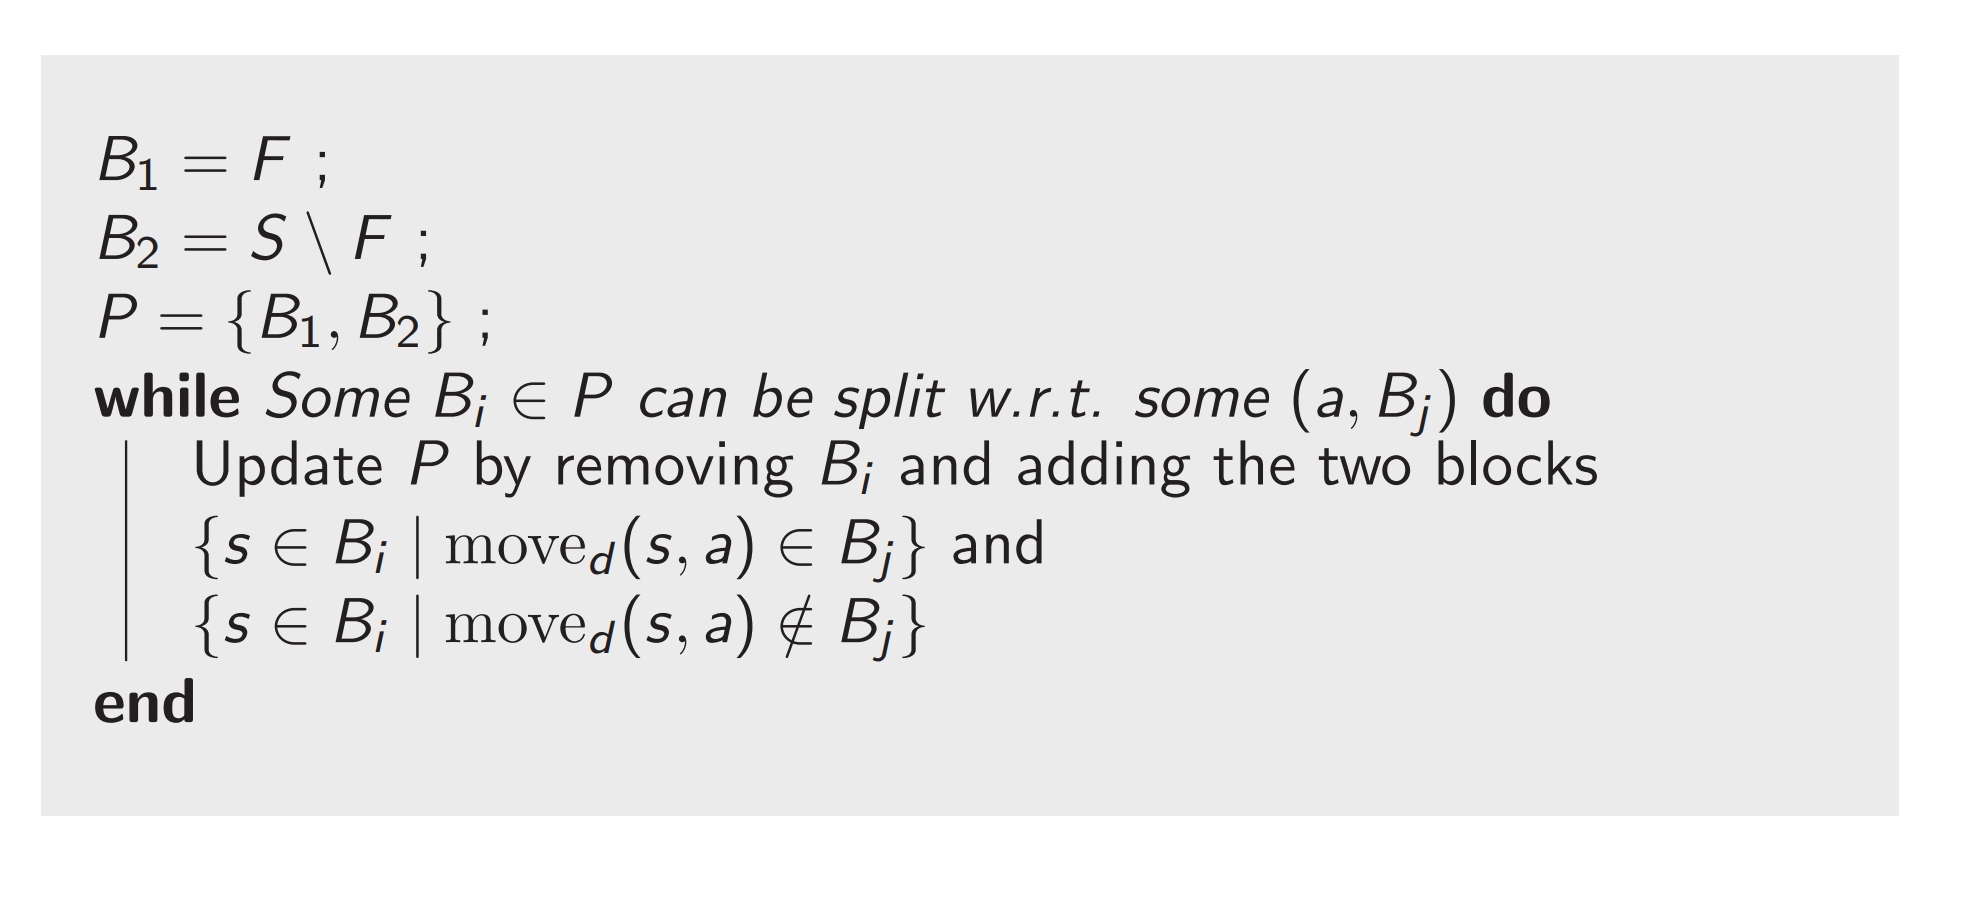
\includegraphics[width=.8\textwidth,keepaspectratio]{algoritmo partiton refinement.png}
% 	\label{partition refinement}
% 	\caption{Pseudocodice}
% \end{figure}
\subimport{assets/pseudocode/}{partition-refinement.tex}

La divisione consiste di \(B_{i}\) considerando \(a,B_{j}\) consiste nel sostituire \(B_{i}\) con due blocchi, \( B_{i1} = {s \in B_{j} \mid move_{d}(s,a)\in B}\) e \( B_{i2} = {s \in B_{j} \mid move_{d}(s,a)\notin B}\)

\subsection{Esercizi sulla minimizzazione DFA}
\subsubsection{Esercizio 1}
Passiamo ad applicare la procedura di minimizzazione ad uno degli esempi già visti in passato.

\begin{figure}[H]
	\centering
    \subimport{assets/figures/}{es1_DFA_minimization.tex}
	\caption{Esercizio 1}
	\label{mindfa-es-1}
\end{figure}

Iniziamo con due blocchi iniziali: \(B_{1}=\{E\}\), dato dallo stato finale, e \(B_{2}=\{A,B,C,D\}\). Notiamo che \((b,B_{1})\) spezza \(B_{2}\), per cui abbiamo due blocchi \(B_{21}=\{D\}\) e \(B_{22}=\{A,B,C\}\). Notiamo ancora che è possibile spezzare \(B_{22}\) in \(B_{221}=\{B\}\) e \(B_{222}=\{A,C\}\). Otteniamo quindi il DFA minimo illustrato in figura \ref{mindfa-es1-sol}. 

\begin{figure}[H]
	\centering
    \subimport{assets/figures/}{sol_es1_DFA_minimization.tex}
	\caption{Soluzione di questo primo esercizio}
  \label{mindfa-es1-sol}
\end{figure}

\subsubsection{Esercizio 2}
Proviamo con questo altro esercizio:

\begin{figure}[H]
	\centering
    \subimport{assets/figures/}{es2_DFA_minimization.tex}
	\caption{DFA dell'esercizio 2}
  \label{mindfa-es-2}
\end{figure}

In questo caso la funzione di transizione non è totale; dobbiamo quindi renderla tale aggiungendo un nodo \(sink\) a cui facciamo arrivare ogni coppia \(stato, simbolo\) mancante dall'equivalente funzione di transizione parziale.

\begin{figure}[H]
	\centering
    \subimport{assets/figures/}{es2_DFA_minimization_total_transition.tex}
	\caption{DFA dell'esercizio 2 con transizione totale}
  \label{minndfa-es-2-tot}
\end{figure}

Dopo aver realizzato questo, iniziamo con gli insiemi \(B_{1}=\{D\}\) e \(B_{2}=\{A,B,D,sink\}\). Possiamo fare uno \emph{split} di \(B_{2}\), in quanto \(\textrm{move}_{d}(A,a) \in B_{2} \) e \(\textrm{move}_{d}(B,a) \notin B_{2} \); da questo split otteniamo i nuovi blocchi \(B_{21}=\{A,sink\}\) e \(B_{22}=\{B,C\}\).

Possiamo fare un ulteriore \emph{split} di \(B_{22}\), poiché \(\textrm{move}_{d}(B,b) \in B_{22} \) e \(\textrm{move}_{d}(C,b) \notin B_{22} \); da questo otteniamo i blocchi \(B_{221}=\{B\}\) e \(B_{222}=\{C\}\).

Infine notiamo che è possibile uno \emph{split} di \(B_{21}\), dal momento che \(\textrm{move}_{d}(A,a) \in B_{221} \) e \(\textrm{move}_{d}(Sink,a) \notin B_{221} \). Otteniamo quindi i blocchi \(B_{211}=\{A\}\) e \(B_{212}=\{sink\}\).
La situazione finale diventa \(B_{1}=\{D\}\), \(B_{211}=\{A\}\), \(B_{212}=\{sink\}\), \(B_{221}=\{B\}\), \(B_{222}=\{C\}\).

Da questo eliminiamo il blocco \(B_{212}\), in quanto il blocco \emph{Sink} non trova posto nel nostro DFA minimo; notiamo però che il DFA minimo che otteniamo è identico a quello di partenza. Il DFA, infatti, era già minimo.  

\begin{figure}[H]
	\centering
    \subimport{assets/figures/}{es2_DFA_minimization.tex}
	\caption{Soluzione Esercizio 2}
  \label{mindfa-es-2-sol}
\end{figure}

\subsubsection{Esercizio 3}
Passiamo ora ad un esercizio più completo. Si richiede di trasformare l'NFA in Fig.\ref{mindfa-es-3} in un DFA e successivamente in un min DFA.
\begin{figure}[htb]
	\centering
  \subimport{assets/figures/}{nfa2.tex}
	\caption{Esercizio 3}
	\label{mindfa-es-3}
\end{figure}
Procediamo dunque, come da prassi, con lo svolgimento della procedura di subset construction per creare un DFA corrispondente. La tabella che riassume tale procedimento è riportata come Tab.\ref{mindfa-es-3-tab}.
\begin{table}[H]
	\centering
	\subimport{assets/tables/}{mindfa-es3-tbl.tex}
	\caption{Tabella per la subset construction}
	\label{mindfa-es-3-tab}
\end{table}
A questo punto dobbiamo costruirne la rappresentazione del DFA, che si può osservare in Fig.\ref{dfa-sc-es-3-mindfa}, e trovarne il minimo.
\begin{figure}
	\centering
    \subimport{assets/figures/}{subset_constr_3_DFA.tex}
	\caption{DFA ottenuto con subset construction}
	\label{dfa-sc-es-3-mindfa}
\end{figure}
Procediamo ora con l’algoritmo di partition refinement per minimizzare il precedente DFA.

Il primo passo è quello di dividere l'insieme \(S\) degli stati in due blocchi: gli stati finali (\(B2\)) e gli stati non finali (\(B1\)).
In questo caso le partizioni sono le seguenti:
\begin{equation*}
    B1 = \{A,B,C,D\} \quad \textrm{e} \quad B2 = \{E,F,G,H\}
\end{equation*}

A questo punto procediamo con le raffinazioni successive. Se all’interno dello stesso blocco troviamo due stati che, tramite una \(a\)-transizione, portano a due blocchi distinti (con \(a\) terminale qualsiasi dell’alfabeto \(\mathcal{A}\)), allora splittiamo questo blocco in due nuovi blocchi nel seguente modo:
\begin{enumerate}
    \item identifichiamo i due stati \(s_1\) e \(s_2\) che con una \(a\)-transizione portano rispettivamente uno in un blocco \(By\) e l’altro in un blocco \(Bz\);
    \item creiamo due nuovi sottoblocchi di \(Bx\): \(Bx_{1}\) conterrà tutti gli stati che da \(Bx\) arrivano a \(By\) con una \(a\)-transizione e \(Bx_{2}\) conterrà tutti gli stati in \(Bx \setminus Bx_{1}\).
\end{enumerate} 
Preme sottolineare che la scelta di quale blocco splittare influisce molto sull’efficienza dell’algoritmo, e gli algoritmi più efficienti svolgono questa scelta in maniera mirata.

Osservo che \(\textrm{move}_d (C,a)\) non ha lo stesso blocco target di \(\textrm{move}_d (A,a) \): infatti, con una \(a\)-transizione da \(A\) raggiungo \(B1\), con una \(a\)-transizione da \(C\) raggiungo \(B2\). Decido quindi di splittare \(B1\) secondo \(\textrm{move}_d (A,a) \). In questo caso il risultato della partizione è il seguente:
\begin{equation*}
    \{A, B\};\; \{C, D\};\; \{E,F,G,H\}
\end{equation*}

Questa nuova partizione è ulteriormente splittabile? Sì! Posso eseguire uno split su \(\textrm{move}_d(A, a)\), dato che attraverso una \(a\)-transizione da \(A\) mi muovo in \(\{A,B\}\), mentre da \(B\) mi muovo in \(\{C,D\}\). Splitto quindi il blocco \(\{A,B\}\) e ottengo questa nuova suddivisione:
\begin{equation*}
    \{A\};\; \{B\};\; \{C, D\};\; \{E,F,G,H\}
\end{equation*}
Ora procediamo ad oltranza con i raffinamenti successivi. Posso splittare su \(\textrm{move}_d(G,b)\) e \(\textrm{move}_d(H,b)\), ottenendo:
\begin{equation*}
    \{A\};\; \{B\};\; \{C, D\};\; \{E,F,H\};\; \{G\}
\end{equation*}
Il prossimo è lo split su \(\textrm{move}_d(C, a)\) e \(\textrm{move}_d(D, a)\), che mi porta ad ottenere:
\begin{equation*}
    \{A\};\; \{B\};\; \{C\};\; \{D\};\; \{E,F,H\};\; \{G\}
\end{equation*}
E ora splitto su \(\textrm{move}_d(E, a)\) e \(\textrm{move}_d(H, a)\):
\begin{equation*}
    \{A\};\; \{B\};\; \{C\};\; \{D\};\; \{E,F\};\; \{H\};\; \{G\}
\end{equation*}
Infine, posso splittare anche su \(\textrm{move}_d(E, a)\) ed \(\textrm{move}_d(F, a)\), arrivando quindi al raffinamento con la seguente forma:
\begin{equation*}
    \{A\};\; \{B\};\; \{C\};\; \{D\};\; \{E\};\; \{F\};\; \{H\};\; \{G\}
\end{equation*}
A questo punto ho raggiunto una partizione in cui tutti i blocchi contengono un solo stato.

In questo caso ho terminato lo svolgimento dell'algoritmo di partition refinement; questo significa che il DFA da cui sono partito (ottenuto da subset construction) era esattamente minimo.

\subsubsection[Tutta da risistemare]{Discussione: “Qual è la scelta ottimale per lo split?”}
Domanda interessante. La discussione, essendo un trivia, verrà trascritta in un secondo momento.
% L’idea alla base dell’algoritmo più efficiente è andare a splittare i blocchi che sono splittabili per archi entranti nei blocchi più piccoli.
% Un algoritmo non efficientissimo ma davvero semplice da scrivere è il seguente
% Algoritmo di Brzozowski
% % min(D) = sub_c(rev(sub_c(rev(D))))
% Precondizione: il DFA può avere un set di stati iniziali
% (non cambia molto per la sub_c: invece di avere lo stato S_0 si ha un insieme di stati T_0, di conseguenza invece che la e-chiusura di S_0 si usa la e-chiusura di T_0)
% Provando ad applicare questo algoritmo su 2/3 automi diversi si dovrebbe arrivare a capire quali sono le scelte migliori per applicare lo split.

\subsection{Dimensione di un DFA}
\begin{lemma}
    Per ogni \(n \in  \mathbb{N}^+\) esiste un NFA con \((n+1)\) stati il cui DFA minimo equivalente ha almeno \(2^n\) stati.
\end{lemma}
\begin{proof}
    Prendiamo ad esempio il linguaggio:
    \begin{equation}
        \mathcal{L} = \mathcal{L}((a\mid b)^\ast a (a\mid b)^{n-1})  
        \label{linguaggio_lemma_limiti_dfa}
    \end{equation}
    Dal momento che è un linguaggio regolare, questo può essere rappresentato utilizzando un automa a stati finiti. Esiste un NFA con esattamente \(n+1\) stati che accetta il linguaggio \(\mathcal{L}\); tale automa è rappresentiato in figura \ref{nfa_lemma_limiti_dfa}.
    \begin{figure}[H]
        \centering
        \subimport{assets/figures/}{dfa_dimension.tex}
        \caption{NFA rappresentante il linguaggio \ref{linguaggio_lemma_limiti_dfa}}
        \label{nfa_lemma_limiti_dfa}
    \end{figure}
    Supponiamo per assurdo che esista un DFA minimo, diaciamo \(\mathcal{D}\), che accetti il linguaggio \(\mathcal{L}\) ed abbia \(k<2^n\) stati.

    Sappiamo esserci esattamente \(2^n\) parole distinte su \(\{a, b\}\) la cui lunghezza è \(n\). Esistono quindi 2 percorsi in \(\mathcal{D}\) tali che:
    \begin{itemize}
        \item la loro lunghezza è \(n\);
        \item compongono rispettivamente le parole \(w_1\) e \(w_2\), con \(w_1 \neq w_2\);
        \item condividono almeno un arco.
    \end{itemize}
    Se non esistessero, allora i nodi sarebbero proprio \(2^n\); di conseguenza per qualche \(x_1\), \(x_2\) e \(x\) vale una delle due opzioni seguenti:
    \begin{itemize}
        \item \(w_1 = x_1 a x \quad \textrm{e} \quad w_2 = x_2 b x\) \textbf{oppure}
        \item \(w_1 = x_1 b x \quad \textrm{e} \quad w_2 = x_2 a x\)
    \end{itemize}
    altrimenti le due parole \(w_1\) e \(w_2\) sarebbero uguali.\\
    Supponiamo in questo caso che sia valida la condizione:
    \begin{equation*}
        w_1 = x_1 a x \quad \textrm{e} \quad w_2 = x_2 b x
    \end{equation*}
    Allora possiamo definire \(w_1'\) in questo modo:
    \begin{equation*}
        w_1' = x_1 a b^{n-1} \in \mathcal{L}(\mathcal{D})
    \end{equation*}
    Di conseguenza, lo stato nuovamente aggiunto da \(w_1'\) in \(\mathcal{D}\) è uno stato finale.
    La precedente affermazione è una contraddizione: lo stato non può essere finale, perché può essere raggiunto anche tramite \(x_2 b b^{n-1}\), ma 
    \begin{equation*}
        x_2 b b^{n-1} \notin \mathcal{L}(\mathcal{D})
    \end{equation*}
    questo è l'assurdo che prova la validità del lemma.
\end{proof}
Tutto il lemma gioca sul fatto che un DFA ha bisogno esattamente di tutti i possibili cammini che siano composti da \(n-1\) alternanze di \(a\) e di \(b\) per esprimere lo stesso linguaggio espresso dall'NFA.

Questo lemma quindi ci offre una stima per il numero minimo di stati di un DFA che rappresenta un certo altro NFA.

\section{Pumping Lemma per linguaggi regolari}
\subsection{Formulazione}
\begin{lemma}
    Sia \(\mathcal{L}\) un linguaggio regolare; allora vale che:
    \begin{itemize}
        \item \(\exists p \in \mathbb{N}^+\) tale che 
        \item \(\forall z \in \mathcal{L}\) tali che \(|z|>p\)
        \item \(\exists \;u, v, w\) tale che
        \begin{itemize}
            \item \(z = uvw\)  e
            \item \(|uv| \le p\)  e
            \item \(|v| \ge 0\)  e
            \item \(\forall i \in \mathbb{N} \; . \; uv^iw \in \mathcal{L}\)
        \end{itemize}
    \end{itemize}
\end{lemma}
\noindent Ovvero, come il lettore avrà ben notato, questo è il corrispettivo del pumping lemma per i linguaggi regolari. Illustriamo ora la dimostrazione di questo lemma.
\begin{proof}
    Dato che \(\mathcal{L}\) è un linguaggio regolare, sappiamo che esiste un DFA \(\mathcal{D} = (S,\mathcal{A},\textrm{move}_d ,s_0, F)\) tale per cui \(\mathcal{L} = \mathcal{L}(\mathcal{D})\).

    Fissiamo quindi \(p=|S|-1\); ciò significa che tutti i cammini che partono da \(s_0\) ed arrivano ad uno stato finale, passando per ogni stato al massimo una volta, hanno lunghezza limitata da \(p\).

    Quindi, se per una parola \(z\) vale \(|z|>p\), allora possiamo scomporre \(z\) in \(z = a_1 \dots a_p z'\) e abbiamo la certezza che almeno uno stato, diciamo \(s^\ast\), sia attraversato più di una volta lungo il cammino \(a_1 \dots a_p\).

    Questo significa che esiste un ciclo in \(\mathcal{D}\) che parte da \(s^\ast\) e torna in \(s^\ast\), e questo ciclo si può indicare come \(a_{i+1} \dots a_j\), con \(i<j\le p\).

    Definiamo ora \(u\), \(v\) e \(w\):
    \begin{itemize}
        \item \(u = a_1 \dots a_i\)
        \item \(v = a_{i+1} \dots a_j\),  (quindi \(v\) rappresenta il ciclo)
        \item \(w = 
        \begin{cases}
            z'                   & \textrm{se} \ j = p\\ 
            a_{j+1} \dots a_pz'  & \textrm{se} \ j < p
        \end{cases}\)
    \end{itemize}

    Quindi possiamo tranquillamente affermare che \(|uv| \le p\) e che la lunghezza di \(v\) è almeno \(1\) (per definizione un ciclo ha almeno un nodo). Inoltre, essendo \(v\) il ciclo, esso è ripetibile (pumping) un numero indefinito di volte, con la garanzia che \(uv^iw\) sia accettato da \(\mathcal{D}\) per ogni valore \(i \in \mathbb{N}\). 
\end{proof}
Abbiamo quindi dimostrato questa versione del pumping lemma per i linguaggi regolari, ora la domanda che sorge spontanea è: per cosa si utilizza questo lemma? Come nel caso dei linguaggi liberi, questo lemma viene utilizzato per dimostrare, tramite contraddizione, che un certo linguaggio \emph{non} è regolare. Quindi, si assume che un dato linguaggio \(\mathcal{L}\) sia regolare, e se si riesce a dimostrare che per quel linguaggio la tesi non è soddisfatta (ovvero il negato della tesi è soddisfatto), allora si può affermare che \(\mathcal{L}\) in realtà non è un linguaggio regolare.

Ripetiamo la tesi, per amor di chiarezza, e ne scriviamo in seguito la negazione.
\begin{labeling}{Negato}
    \item[Tesi] 
    \(\exists p \in \mathbb{N}^+ . \;\forall z \in \mathcal{L}:|z|>p . \; \exists \;u, v, w . \; P\), \\ 
    dove \\
    \(P \equiv (z = uvw \textrm{ and } |uv| \le p \textrm{ and } |v| \ge 0 \textrm{ and } \forall i \in \mathbb{N} . \; uv^iw \in \mathcal{L}) \)
    \item[Negato]
    \(\forall p \in \mathbb{N}^+ . \;\exists z \in \mathcal{L}:|z|>p . \; \forall \;u, v, w . \; Q\), \\
    dove \\
    \(Q \equiv (z = uvw \textrm{ and } |uv| \le p \textrm{ and } |v| \ge 0) \implies (\exists i \in \mathbb{N} . \; uv^iw \notin \mathcal{L}) \) 
\end{labeling}

\subsection{Applicazioni del pumping lemma per linguaggi regolari}
Vediamo subito come possiamo applicare il lemma per dimostrare la seguente affermazione:
\begin{equation}
    \mathcal{L} = \{a^n b^n \mid n>0\} \quad \textrm{non è regolare.}
    \label{pl_regular_languages_ex_1}
\end{equation}
Prima di proseguire con la dimostrazione formale, proviamo a spiegare che intuizione potrebbe dirci che ci troviamo davanti ad un linguaggio non regolare.

Se \(\mathcal{L}\) fosse un linguaggio regolare dovrebbe essere possbile rappresentarlo con un NFA o un DFA. Proviamo quindi a immaginare il DFA che riconosce questo linguaggio, come dovrebbe essere? Per bilanciare il numero di \(b\) e di \(a\) dovrebbe in qualche modo obbligare l’inserimento di una \(b\) per ogni \(a\) inserita in precedenza, ma questo non si può fare a meno di inserire infiniti stati, il che è impossibile.

Procediamo quindi con la dimostrazione tramite pumping lemma. Supponiamo \(\mathcal{L}\) regolare e prendiamo \(p\) intero positivo arbitrario (il negato della tesi deve valere per ogni \(p\)). Ora, costruiamo la parola \(z=a^p b^p\); abbiamo che \(|z|>p\).
Osserviamo che:
\begin{equation*}
    \forall \; u,v,w \ \textrm{se} \ (z = uvw \quad \textrm{e} \quad |uv| \le p \quad \textrm{e} \quad |v| > 0)
\end{equation*}
Sappiamo inoltre che:
\begin{itemize}
    \item la componente \(v\) contiene almeno una \(a\) (da \(|v| > 0\));
    \item la componente \(v\) può contenere solamente \(a\) (altrimenti violerebbe \(|uv| \le p\)).
\end{itemize}
Se noi ora definiamo \(j > 0\) tale per cui 
\begin{equation*}
    uv^2w = a^pa^jb^p 
\end{equation*}
abbiamo che \(uv^2w \notin \mathcal{L}\), il che contraddice il pumping lemma per i linguaggi regolari.

Abbiamo quindi dimostrato per contraddizione del pumping lemma per linguaggi regolari che l'affermazione in equazione \ref{pl_regular_languages_ex_1} è verificata.

\subsection{Esercizi sul riconoscimento di linguaggi regolari}
\subsubsection{Esercizio 1}
Sia \(\mathcal{L}_1\) il linguaggio delle parole su \(\{a, b\}\) con un numero dispari di occorrenze di \(b\). \(\mathcal{L}_1\) è regolare?
\begin{figure}[H]
    \centering
    \subimport{assets/figures/}{regual_recognition_es1.tex}
    \caption{DFA che riconosce un numero dispari di occorrenze di \(b\) in un linguaggio su \(\{a,b\}\)}
    \label{b_dispari}
\end{figure}

Proponiamo di seguito delle espressioni regolari e dei DFA che sono stati selezionati durante la lezione con una breve spiegazione a riguardo 

\begin{itemize}
    \item l'espressione regolare \((a^*(bb)^*)^* b(a^*(bb)^*)^*\) non può denotare il linguaggio descritto poiché \(ababab \notin \mathcal{L}_1\).
    \item definiamo un automa con due stati \(A\) iniziale e \(B\) finale. \(A\) presenta una \(a\)-transizione in \(A\) ed una \(b\)-transizione in \(B\) mentre \(B\) ha una \(a\)-transizione in \(B\) e una \(b\)-transizione in \(A\). Notare che lo stato \(A\) rappresenta il caso in cui sono state lette un numero pari di \(b\) mentre \(B\) quello in cui sono state lette un numero dispari di \(b\): nel caso iniziale, infatti, si è obbligati ad aggiungere almeno una \(b\) per raggiungere lo stato finale ma, nel caso in cui si voglia aggiungere un'altra \(b\), è necessario ritornare nello stato \(A\) e rifare il procedimento descritto. Considerando che in entrambi gli stati è possibile mettere un numero arbitrario di \(a\), possiamo dichiarare questa soluzione come corretta.
    \item l'espressione regolare \((a^*(b)a^*)(a^*(b)a^*(b)a^*)^*\) sembrerebbe essere corretta in quanto sicuramente accetterò parole composte da almeno una \(b\) e un numero arbitrario di \(a\) prima e dopo; nel caso in cui volessi aumentare il numero di \(b\), sono obbligato a farlo a coppie con la possibilità di interporre un numero arbitrario di \(a\) prima, in mezzo o alla fine. 
\end{itemize}

In questo caso, visto che siamo stati in grado di trovare un DFA con un numero finito di stati, possiamo affermare che \(\mathcal{L}_1\) è un linguaggio regolare. Come possiamo però essere certi del fatto che, ad esempio, l'espressione regolare \((a^*(b)a^*)(a^*(b)a^*(b)a^*)^*\) denoti il linguaggio \(\mathcal{L}_1\) e che quindi sia anch'essa soluzione al quesito? Il modo corretto di procedere è il seguente:

\begin{enumerate}
    \item si utilizza la \emph{Thompson's Construction} per generare l'NFA corrispondente;
    \item si applica l'algoritmo di \emph{Subset Construction} per trasformare l'NFA in un DFA;
    \item si applica l'algoritmo per la \emph{DFA minimization} (aggiungendo dunque lo stato sink se necessario) per ridurre il numero di stati;
    \item si osserva se il DFA ridotto è in realtà un isomorfismo del DFA proposto come soluzione (in questo caso il DFA proposto come soluzione è sicuramente minimo, in quanto ha solamente due stati).
\end{enumerate}

\noindent Notare che in questo caso una soluzione possibile (proposta dalla professoressa) è \((b a^*b \mid a)^* ba^*\)

\subsubsection{Esercizio 2}
Sia \(\mathcal{L}_2\) il linguaggio delle parole su \(\{a, b\}\) con un numero pari di occorrenze di \(a\). \(\mathcal{L}_2\) è regolare?
\begin{figure}[H]
    \centering
    \subimport{assets/figures/}{regual_recognition_es2.tex}
    \caption{DFA che riconosce un numero pari di occorrenze di \(a\) in un linguaggio su \(\{a,b\}\)}
    \label{a_pari}
\end{figure}

Per rispondere a tale quesito si potrebbe pensare di costruire un DFA con lo stesso ragionamento di prima: uno stato il caso in cui le occorrenze di \(a\) sono pari mentre l'altro in cui sono dispari.

Poiché \(0\) è considerato pari, in questo caso lo stato iniziale coincide con quello finale. Le transizioni devono essere opportunamente costruite, per cui se voglio aggiungere una \(a\) alla mia parola sono costretto a seguire una \(a\)-transizione in uno stato non finale per poi tornare in quello finale con un'ulteriore \(a\)-transizione, in modo da assicurare che le condizioni siano rispettate. Ovviamente, deve esservi sempre la possibilità di inserire un numero arbitrario di \(b\) tra le varie occorrenze di \(a\), per cui in entrambi gli stati si ha una \(b\)-transizione sullo stesso stato. Analogamente all'esercizio precedente si ha che \(\mathcal{L}_2\) è un linguaggio regolare. In questo caso l'espressione regolare proposta è stata \((b^*ab^*ab^*)^*\) .
% (P.S. ho provato a fare l'isomorfismo di questo grafo e non viene mai nella vita identico a quello precedente, potrei avere tranquillamente sbagliato ma l'abbiamo fatto in 3 e non risulta quindi o c'è qualcosa che mi sfugge o IDK)

\subsubsection{Esercizio 3}  
Sia \(\mathcal{L}_3\) il linguaggio delle parole su \(\{a, b\}\) con un numero dispari di occorrenze di \(b\) \textbf{oppure} un numero pari di occorrenze di \(a\). \(\mathcal{L}_3\) è regolare?

Una soluzione tanto banale quanto efficace consiste nel utilizzare la Thompson's Construction per poter concatenare gli automi descritti negli esercizi precedenti con l'operazione di \emph{alternanza}. A livello formale questo si traduce come:
\begin{equation*}
    \mathcal{L}(r_1 \mid r_2) = \mathcal{L}(r_1) \cup \mathcal{L}(r_2)
\end{equation*}
\begin{figure}[H]
    \begin{minipage}[b]{0.4\textwidth}
        \centering
        \subimport{assets/figures/}{regual_recognition_es3_a.tex}
        \subcaption{NFA che riconosce un numero dispari di occorrenze di \(b\) \textbf{oppure} un numero pari di occorrenze di \(a\) in un linguaggio su \(\{a,b\}\)}
    \label{nfa-b_odd-or-a_even}
    \end{minipage}
    \hfill
    \begin{minipage}[b]{0.4\textwidth}
        \centering
        \subimport{assets/figures/}{regual_recognition_es3_b.tex}
        \subcaption{DFA che riconosce un numero dispari di occorrenze di \(b\) \textbf{oppure} un numero pari di occorrenze di \(a\) in un linguaggio su \(\{a,b\}\)}
        \label{dfa-b_odd-or-a_even}
    \end{minipage}
    \caption{}
\end{figure}
Essendo che \(\mathcal{L}_1\) e \(\mathcal{L}_2\) sono linguaggi regolari, l'unione dei due così descritta non può che essere anch'essa un linguaggio regolare.

\subsubsection{Esercizio 4}
Riprendiamo la formulazione dell'esercizio precedente; nel caso in cui fosse stato richiesto di verificare un linguaggio dove valessero \textbf{entrambe} le condizioni precedenti avremmo dovuto procedere in modo diverso. Sono dati i seguenti casi:
\begin{itemize}
    \item abbiamo un numero di \(a\) pari e di \(b\) pari;
    \item abbiamo un numero di \(a\) pari e di \(b\) dispari;
    \item abbiamo un numero di \(a\) dispari e di \(b\) pari;
    \item abbiamo un numero di \(a\) dispari e di \(b\) dispari.
\end{itemize}
Ovviamente il nostro stato iniziale non può essere altro che quello dove si hanno \(0\) occorrenze di \(a\) e di \(b\) (il primo descritto), mentre lo stato finale dovrà per forza essere il secondo dell'elenco. Dunque quello che abbiamo appena immaginato di costruire è un'automa che possiede \(4\) possibili stati di cui soltanto uno deve essere considerato quello finale. 

\begin{figure}[H]
    \centering
    \subimport{assets/figures/}{regual_recognition_es4.tex}
    \caption{DFA che riconosce un numero dispari di occorrenze di \(b\) \textbf{e} un numero pari di occorrenze di \(a\) su un linguaggio su \(\{a,b\}\)}
    \label{dfa-b_odd-and-a_even}
\end{figure}

Sicuramente l'idea precedente è corretta, ma c'era un altro modo per arrivare direttamente alla soluzione senza dover fare un ragionamento di quel tipo, ma pensando invece all'intersezione: immaginiamo di avere una parola \(w\) a disposizione e di poterci contemporaneamente muovere su entrambi i cammini degli automi descritti come soluzioni di \(\mathcal{L}_1\) e di \(\mathcal{L}_2\). Continuiamo a spostarci eseguendo le transizioni coerentemente alla parola \(w\) scelta, fino a che non arriviamo al carattere terminatore. A questo punto sono dati due casi:
\begin{enumerate}
    \item se mi trovo in entrambi gli automi su uno stato finale allora \(w \in \mathcal{L}\)
    \item se uno dei due stati su cui mi trovo non è uno stato finale allora \(w \notin \mathcal{L}\)
\end{enumerate}
\begin{figure}[H]
    \begin{minipage}[b]{0.4\textwidth}
        \centering
        \subimport{assets/figures/}{regual_recognition_es4-2_a.tex}
        \subcaption{step by step by mike by bisognaspiegarlo}
        \label{pl-es4-sbs_1}
    \end{minipage}
    \hfill
    \begin{minipage}[b]{0.4\textwidth}
        \centering
        \subimport{assets/figures/}{regual_recognition_es4-2_b.tex}
        \subcaption{step by step by mike by bisognaspiegarlo 2}
        \label{pl-es4-sbs_2}
    \end{minipage}

    \begin{minipage}[b]{0.4\textwidth}
        \centering
        \subimport{assets/figures/}{regual_recognition_es4-2_c.tex}
        \subcaption{step by step by mike by bisognaspiegarlo 3}
        \label{pl-es4-sbs_3}
    \end{minipage}
    \hfill
    \begin{minipage}[b]{0.4\textwidth}
        \centering
        \subimport{assets/figures/}{regual_recognition_es4-2_d.tex}
        \subcaption{step by step by mike by bisognaspiegarlo 4}
        \label{pl-es4-sbs_4}
    \end{minipage}
    \caption{}
\end{figure}

Per poter semplificare la procedura possiamo immaginare di fare il prodotto cartesiano degli stati dei due automi.

\section{Proprietà di chiusura nei linguaggi regolari}

I linguaggi regolari sono chiusi rispetto alle seguenti operazioni:
\begin{itemize}
	\item unione;
	\item concatenazione;
	\item complementazione;
	\item intersezione.
\end{itemize}
Andiamo a vedere più da vicino le motivazioni per ciascuna di queste.

\paragraph{Unione}
Se prendiamo due linguaggi regolari e ne operiamo l'unione, il risultato di questa è ancora un linguaggio regolare. Come nel caso precedente, essendo che i linguaggi sono regolari, allora è possibile costruire un DFA sia per il primo che per il secondo; se a questo punto si prendono i due automi così costruiti e li si lega tramite una \(\epsilon\)-transizione, per l'operazione di \emph{alternanza} si ottiene nuovamente 
un linguaggio regolare.

\paragraph{Concatenazione}
È possibile eseguire l'operazione di \emph{concatenazione} della Thompson's Construction e ottenere ancora una volta un'automa che denota un linguaggio regolare.

\paragraph{Complementazione}
Se \(\mathcal{L}\) è un linguaggio regolare su un certo alfabeto \(\mathcal{A}\), la complementazione è data dal linguaggio delle parole su \(\mathcal{A} \setminus \mathcal{L}\). Se un linguaggio è regolare allora anche il suo complemento è regolare. 

\paragraph{Intersezione}
È derivabile dall'unione utilizzando le regole di \emph{De Morgan}: 
\begin{equation*}
    \mathcal{L}_1 \cap \mathcal{L}_2 = \lnot (\lnot (L1 \cap L2)) = \lnot (\lnot \mathcal{L}_1 \cup \lnot \mathcal{L}_2)
\end{equation*}

In precedenza abbiamo visto l'automa che riconosce \(\mathcal{L}_2\), ovvero che accetta tutte quelle parole dove \(a\) occorre un numero pari di volte. Il complementare di tale automa corrisponde a quello per cui si hanno parole con un numero dispari di occorrenze. Utilizzando l'automa che denota \(\mathcal{L}_2\), vi è la possibilità di applicare una particolare operazione per trasformarlo nel suo complementare? Sì, è possibile: basta semplicemente rendere finali tutti quegli stati che prima non lo erano e, simmetricamente, non finali tutti quelli che prima lo erano.

Relativamente questo procedimento è però necessario fare una precisazione: tale metodo funziona solamente se il DFA presenta una funzione di transizione \textbf{totale}: intuitivamente, è necessario riconoscere tutte quelle parole che non appartengono al linguaggio regolare in quanto queste apparterranno al linguaggio del DFA complementare; se per assurdo si avesse la mancanza di una \(a\)-transizione (non fondamentale nel primo DFA) non si avrebbe la possibilità di costruire il set completo delle parole.

\end{document}